\subsubsection{Estrutura}

% SLIDE DE ESTRUTURA
\begin{frame}
\frametitle{Estrutura}

\begin{figure}
\centering
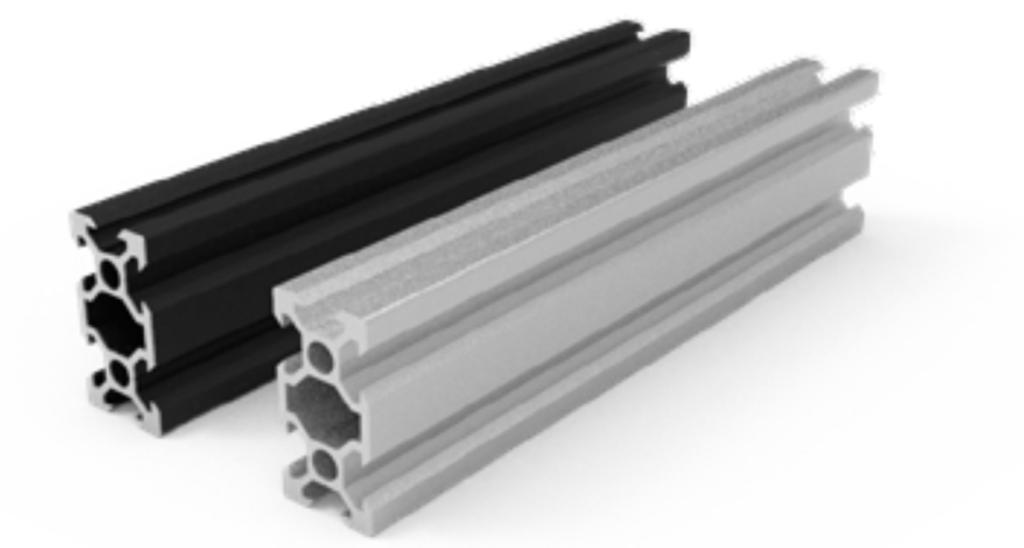
\includegraphics[scale = 0.15]{figs/p20x40p}
\end{figure}

\begin{figure}
\centering
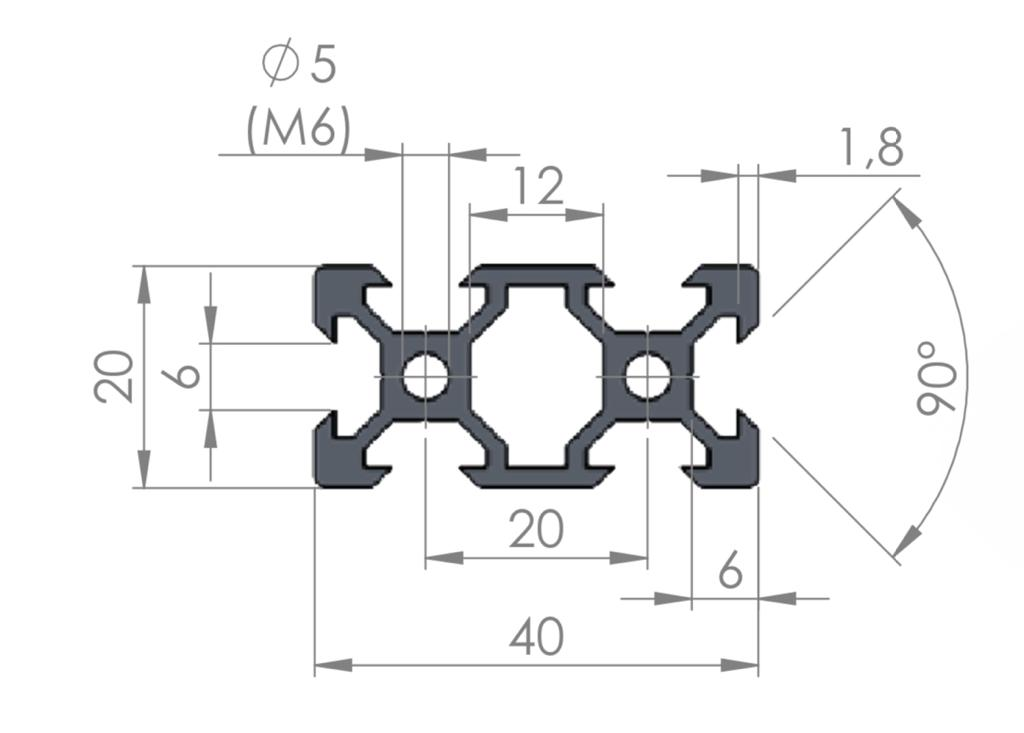
\includegraphics[scale = 0.15]{figs/p20x40d.jpeg}
\end{figure}
    
\end{frame}
    
% SLIDE DE ESTRUTURA
\begin{frame}
\frametitle{Estrutura}

\begin{figure}
\centering
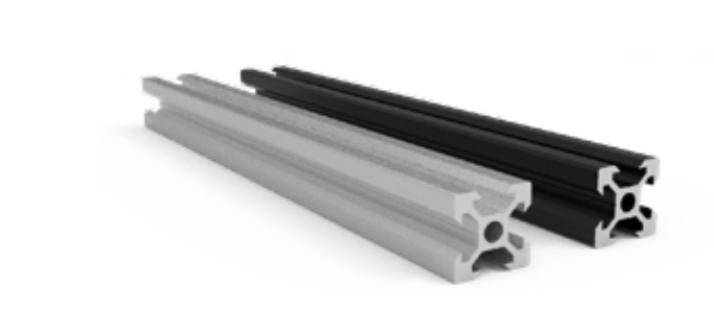
\includegraphics[scale = 0.25]{figs/p20x20p}
\end{figure}

\begin{figure}
\centering
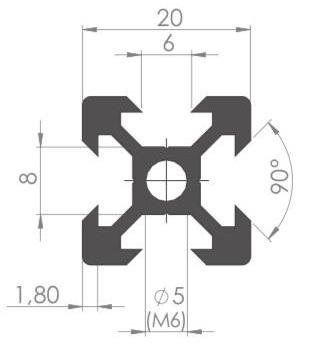
\includegraphics[scale = 0.45]{figs/p20x20d}
\end{figure}
    
\end{frame}

% SLIDE DE ESTRUTURA
\begin{frame}
\frametitle{Estrutura}

\begin{figure}
\centering
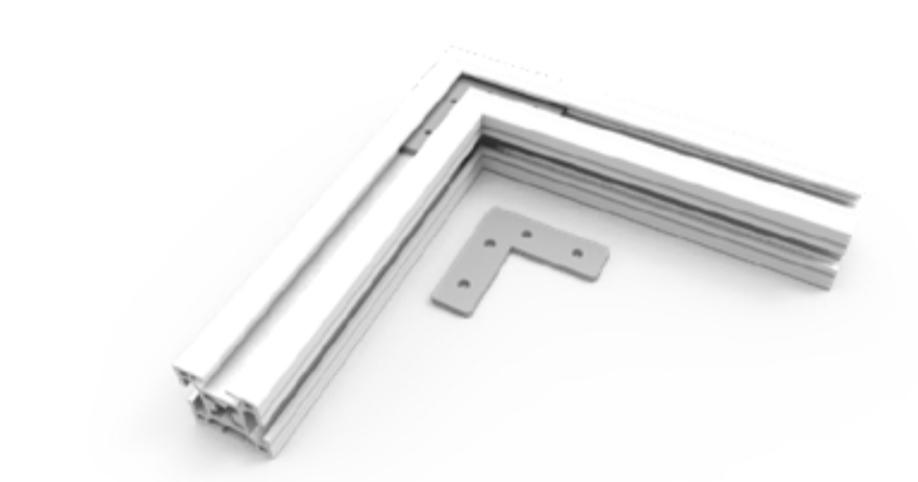
\includegraphics[scale = 0.15]{figs/pconexao90p}
\end{figure}

\begin{figure}
\centering
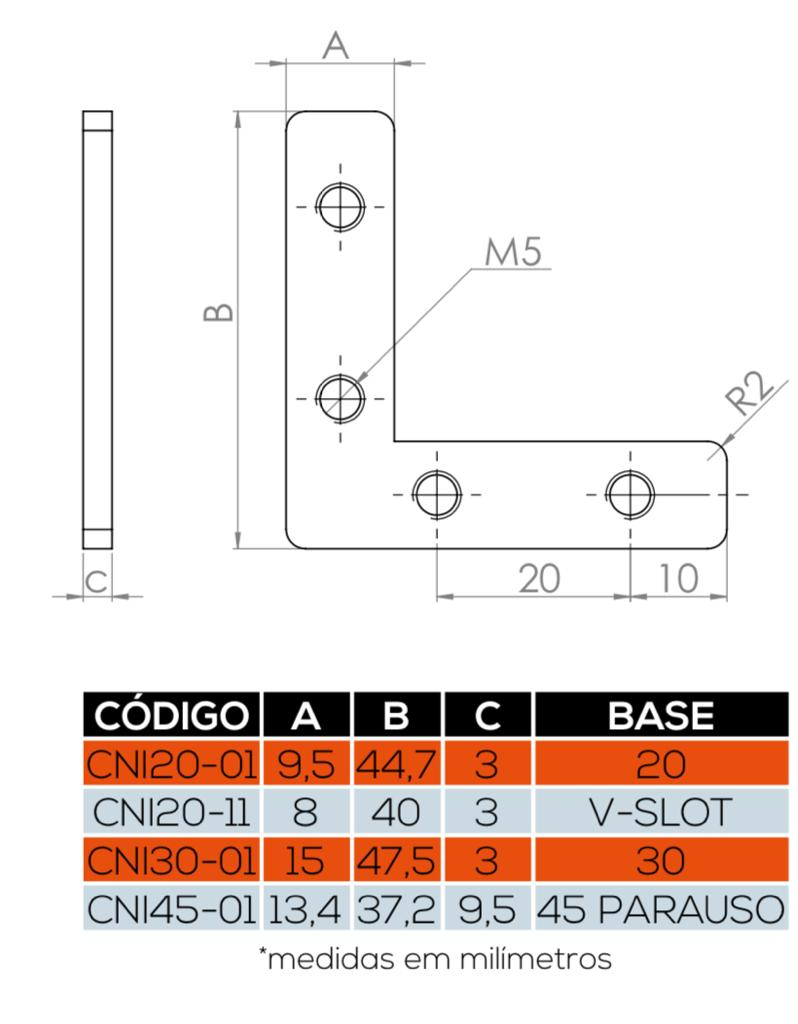
\includegraphics[scale = 0.15]{figs/pconexao90d}
\end{figure}
    
\end{frame}

% SLIDE DE ESTRUTURA
\begin{frame}
\frametitle{Estrutura}

\begin{figure}
\centering
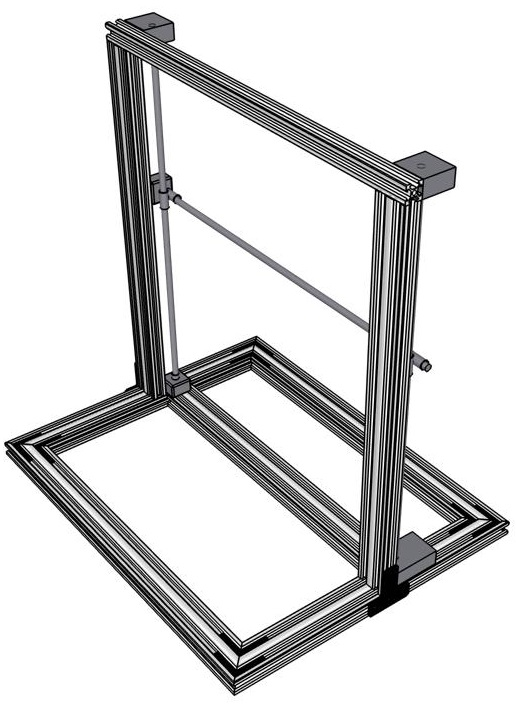
\includegraphics[scale = 0.4]{figs/estruturamesa}
\end{figure}  

\end{frame}
    
% SLIDE DE ESTRUTURA
\begin{frame}
\frametitle{Estrutura}

\begin{figure}
\centering
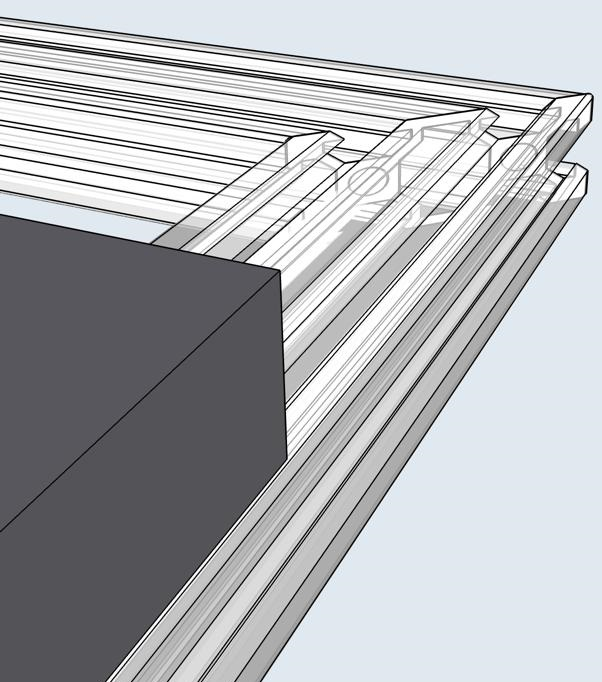
\includegraphics[scale = 0.4]{figs/detalhe45}
\end{figure}  
    
\end{frame}

% SLIDE DE ESTRUTURA
\begin{frame}
\frametitle{Estrutura}

\begin{figure}
\centering
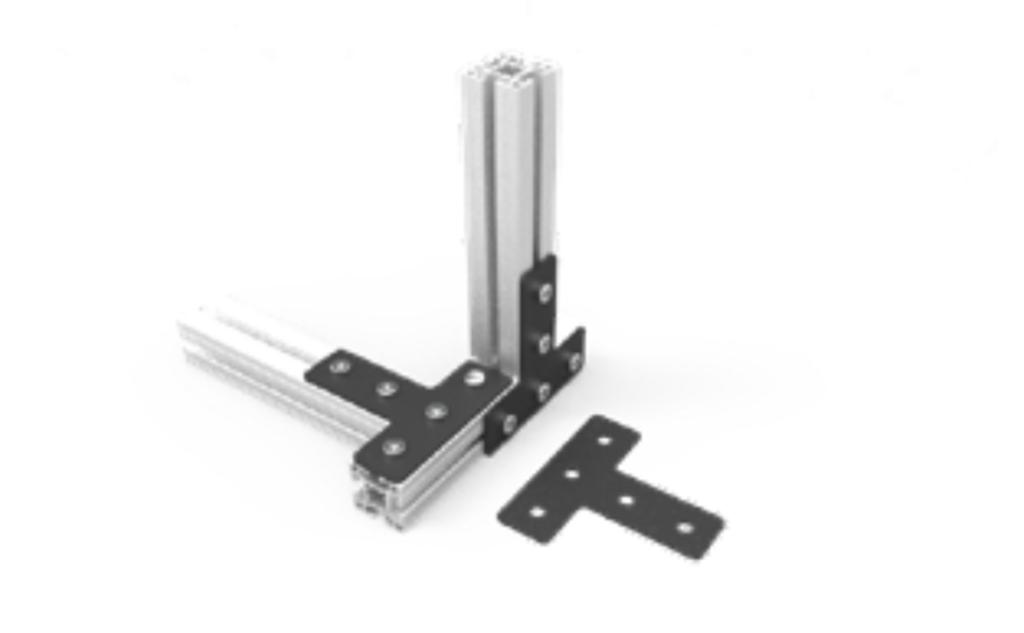
\includegraphics[scale = 0.10]{figs/placatp}
\end{figure}

\begin{figure}
\centering
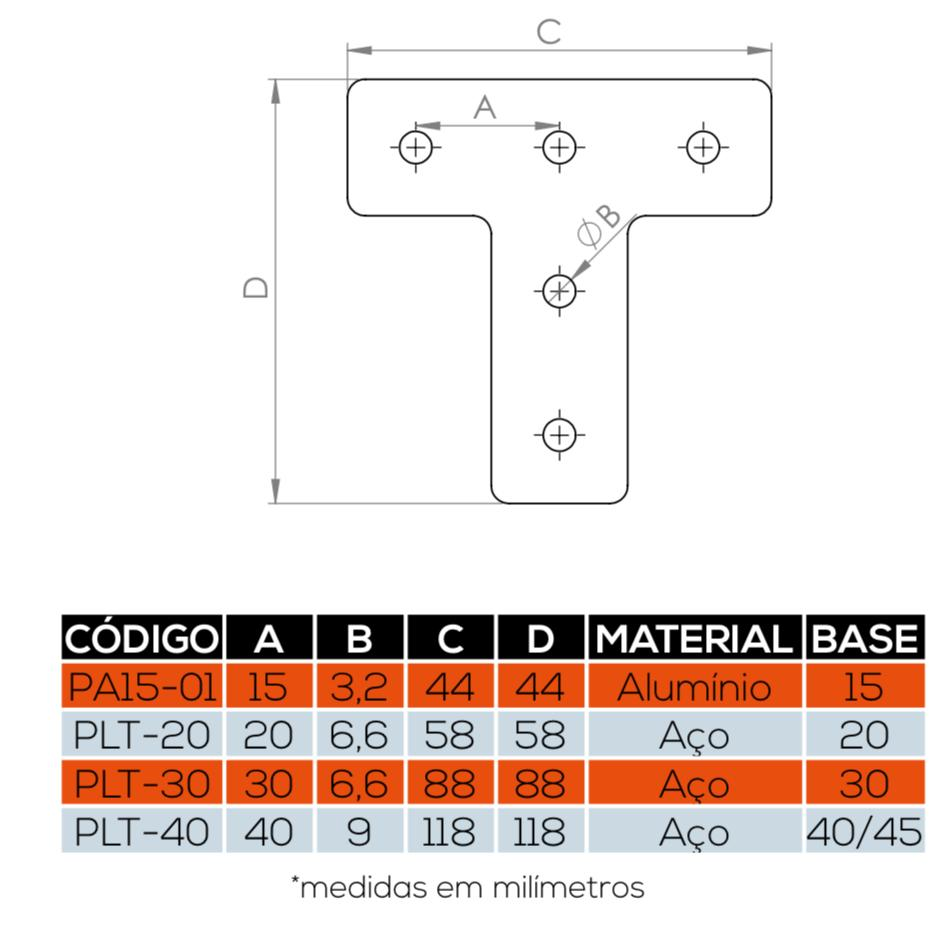
\includegraphics[scale = 0.10]{figs/placatd}
\end{figure}
    
\end{frame}
